\Chapter{Megvalósítás}

\begin{figure}[h]
\centering
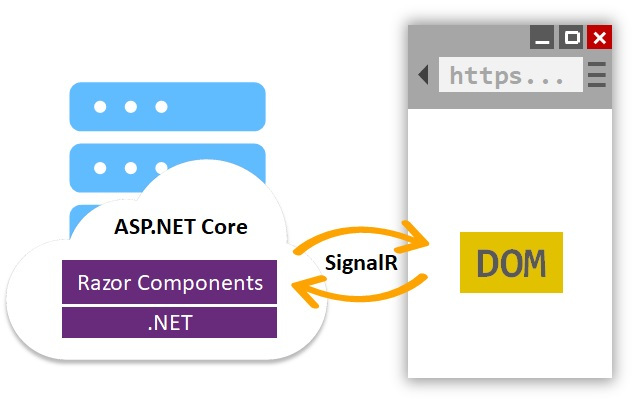
\includegraphics[scale=0.5]{images/blazor.jpg}
\caption{Blazor Server. Forrás:https://docs.microsoft.com/en-us/aspnet/core/blazor/?view=aspnetcore-6.0}
\label{fig:blazor}
\end{figure}

\Section{ASP.NET Core Blazor}
A megvalósításra felhasznált technológia végül a ASP.NET Core Blazor lett, ami egy .Net keretrendszer komplex, interaktív webalkalmazások létrehozására. Lényege, hogy a weboldalhoz  JavaScript helyett C\# kódot írhassunk. Kicsit pontosabban, szinte minden frontend logikához C\# kód a megoldás HTML elemek elrendezésétől a weboldal navigálásán át fájlok feltöltéséig.

Jelenleg 2 verziója támogatott, Blazor Server ahol egy szerver alkalmazásban fut a kód, és Blazor WebAssembly, ahol közvetlenül a böngészőben. Ebben a projektben a Blazor Server-t választottam a nagyobb támogatottsága miatt.

\Section{Razor komponensek}
Blazor alkalmazások jelentős részben Razor komponensekből épülnek fel. Egy komponens az UI egy önálló része, ami tartalmazhat feldolgozó logikát hogy dinamikusan viselkedhessen. Komponenseket lehet többször felhasználni, egymásba ágyazni, vagy Razor oldalakban felhasználni (egy komponens akár önmagában is lehet Razor oldal). Egy Razor komponens tartalmaz HTML elemeket és @ jellel ellátott C\# kifejezéseket, amik lehetnek direktívák, logikák, vagy akár komplex kód részek is.

\Section{Routing, SignalR, and Dependency Injection}
Routing, azaz útvonal választás az a folyamat, ahogy a szerver a bejövő HTTP kéréseket az alkalmazás végrehajtható végpontjaihoz párosítja. Az ASP.Net ezt szinte automatikusan teszi meg, a megfelelő kérést a megfelelő Razor oldalra irányítja, miután megadjuk neki a kellő feltérképezési beállítást. 

Viszont nem minden interakció eredményez HTTP kérést, a legtöbb kommunikáció a weboldal és a szerver között SignalR segítségével történik. A SignalR egy nyílt forrású könyvtár ami lehetővé teszi a valós idejű kommunikációt a szerver és a weboldal között. Ha a UI egy interaktív elemét "megpiszkájuk", a weboldal SignalR-en át átküldi az esemény(eke)t a szervernek, a szerver végrehajtja a kérést, majd szintén SignalR-en keresztül visszaküldi a UI frissítéseket.

A Dependency Injection egy szoftverdizájnbeli minta, aminek lényege, hogy megfordítja az irányítást elemek és függőségeik között. ASP.NET-ben ez annyit jelent, hogy az osztályok vagy komponensek ahelyett hogy önmaguk hoznák létre vagy konstruktorukban kapják meg a függőségeiket, egy úgynevezett DI konténer hozza őket létre. 3 féle módon lehet a függőségeket kezelni:
\begin{itemize}
\item\textbf{Transient Object} Minden esetben új és egyedi objektumot hoz létre.
\item\textbf{Scoped Object} Egy kérésen belül ugyanazt az objektumot biztosítja.
\item\textbf{Singleton Object} Minden esetben ugyanaz a (meglévő) objektum.
\end{itemize}
Ez az alkalmazás főleg Singleton-okat használ szolgáltatások biztosítására és közös adatok elérésére. Mivel végig egy felhasználó dolgozik egy munkamenetben, nincs szükség limitálni a függőségek élettartamát és elérhetőségét.

\Section{Hardware Service}
A .NET Core hivatalosan egy multiplatform alkalmazás, de sajnos még vannak olyan részei amik jelenleg még csak a Windows-t támogatják. A Hardware elemzésére a hivatalosan támogatott módszer a WMI (Windows Management Instrumentation) használata, nevéből adódóan jelenleg csak Windows-on elérhető, ezért más operációs rendszerek esetében az alkalmazás hamis, kitalált adatokkal dolgozik, amíg a Microsoft ki nem terjeszti a támogatását Linuxra és társaira.

\Section{Navigation Menu}
Az alkalmazásban a navigáció különböző oldalak között az oldalsó navigációs menün keresztül történik. Ennek az az érdekessége, hogy a menüpontok csak akkor jelennek meg, ha tartalmuk készen áll. Itt olyan probléma merült fel, hogy a menü nem frissül magától, ezért be kellett iktatni egy új szolgáltatót, a MenuService-t. A MenuService feladata egy esemény kezelése. Ha a programban olyan változás történik ami hatással van a menüre, a szolgáltatás meghívja az eseményt, amit a menü már észlelni tud és lereagálja. 

\Section{Architeture oldal}
Az Architecture oldal fő és egyetlen eleme egy Canvas, pontosabban egy Blazor Extension Canvas, ami azért előnyös mert könnyen manipulálható C\# kóddal. Ez a komponens miután létrehozza a Canvas-t, megrajzolja a Hardware Service által szolgáltatott adatokat, mint a fizikai memória, CPU, GPU. Az egyszerűség kedvéért fix méretű Canvas-al dolgozik, így pixel pontosan meg tudja rajzolni az entitásokat és a kapcsolatokat. A használt eszközöket zöld színnel jelzi.

\Section{Analysis}
Ez az egyik fő alkotóeleme a programnak, itt megvizsgáljuk a beolvasott fájlt, és sorról sorra végigmegyünk rajta OpenCL elemeket kutatva. 

Első lépésben megvizsgálja hogy a program CPU-nak vagy GPU-n fut-e és ez alapján megállapítja a megfelelő Compute Unit mennyiséget, ami processzor esetén a logikai szálakkal egyenértékű. Viszont videokártya esetén ez egy sokkal összetettebb probléma, nem lehet ilyen egyszerűen megmondani a számítási egységek mennyiségét. Például egy Nvidia 1080 videókártyában 2560 shading unit,160 texture mapping unit, és 64 ROP egység található. Ez egyrészt nem látható a WMI számára, másrészt ebből kikövetkezthetetlen a tényleges OpenCL számítási egységek száma. És ettől csak bonyolultabb esetek vannak, lehetnek CUDA magok vagy Tensor magok is, lehet integrált videókártya ami bizonyos erőforrásokon a processzorral osztozik, más gyártású, például AMD videókártyák pedig teljesen más felépítésűek is lehetnek. Ha sikerülne is megállapítani a számítási egységek számát, 3000+ számítási szálat nem lehet jól vizualizálni, ezért videókártya esetén az ábrázolás céljából a program egy kitalált 4 számítási egységgel fog dolgozni.

Második lépésben összegyűjti az OpenCL elemeket egy listában és megadja a hozzájuk tartozó számítási egység számát. Ez lehet:
\begin{itemize}
\item\textbf{0} , ami azt jelenti hogy egy szálon fut szekvenciálisan,
\item\textbf{1,2,3.....} , ami a hozzá tartozó tényleges számítási egység száma,
\item\textbf{-1} , ami azt jelöli hogy az összes elérhető számítási egységen párhuzamosan történik.
\end{itemize}

\Section{Code oldal}
Ez a második megjelenítő felület. 2 egymás mellett lévő konténerből épül fel.
A baloldali konténerben egy dinamikus táblázat foglal helyet ami a már elemzett objektumokat jeleníti meg Gannt diagram formában. A diagram bal oldalán a végrehajtás lépésének indexe, tetején pedig a számítási egységek sorszámai szerepelnek, plusz a 0-s oszlop ami a szekvenciális futást jelzi. A diagram a számítási egységeknek megfelelően az oldal betöltésekor dinamikusan töltődik fel elemekkel. A diagram elemi html gombok, amik tartalmazzák az elemek neveit, valamint a megfelelő funkciókat. Szükséges a ciklusváltozó "elfogása" az ii változó által, ellenkező esetben a függvények mindannyian az alap ciklusváltozó végső értékét fogják használni.

\begin{cpp}
@for(int i = 0; i < Analyzer.myElements.Count; i++)
 {
   int ii = i;
   <tr>
      <td>@(i+1)</td>
      @for(int j = 0; j < Analyzer.CUs+1; j++)
        {
          <td style="min-width:50px">
          @if (j==Analyzer.myElements[ii].ComputeUnit | (j!=0 &
               -1==Analyzer.myElements[ii].ComputeUnit))
             {
                <button title=@Analyzer.myElements[ii].Name @onclick="()
                =>{ChangeColor(Analyzer.myElements[ii].Index);ScrollTo
                Analyzer.myElements[ii].Index);}">@(i+1)</button>
             }
          </td>
        }
   </tr>
 }
\end{cpp}


A második konténerben, vagyis az oldal jobb oldalán magát a forráskódot jelenítjük meg sorokra osztva, az üres sorokat még a feldolgozás közben eltávolítva. Minden sor külön paragrafus elem, id-val ellátva, hogy lehessen rájuk hivatkozni. Itt lesz szerepe a Gannt diagram gombjainak. Egy gomb megnyomásakor a hozzá tartozó elem színe zöldre, a többi pedig fehérre vált. Ez a fent említett SignalR-en keresztül zajlik, majd ugyanitt frissül az oldal és a megfelelő kódsor paragrafusa ténylegesen zöldre vált. Emellett a böngésző a megfelelő helyre is teker, ami JavaScript-et igényel. A program ekkor JavaScript Interop használatával meghív egy JS függvényt ami elvégzi a kérést.

\begin{cpp}
jsRuntime.InvokeAsync<bool>("test","line{" + (i-8) + "}");
\end{cpp}


%\begin{verbatim}
%$ some commands with arguments
%1 2 3 4 5
%$ _
%\end{verbatim}


